\documentclass[10pt,a4paper]{beamer}

%\usepackage[applemac]{inputenc}
\usepackage[ngerman]{babel}
\usepackage[utf8]{inputenc}
\usepackage{times}
\usepackage{graphicx}
\usepackage{setspace} %Zeilenabstand?
\usepackage{wrapfig} %Benoetigt fuer Textumflossene Bilder
\usepackage{hyperref}
\usepackage{marvosym} %Symbol Link
\usepackage{fontawesome5}
%%%%%%%%%%%%%%%%%%%%%%%%%%%%%%%%%%%%%%%%%%%%%%%%%%%%%%%%%%%%%%%%%%%%%%%%%%%%%%%%
\usetheme{Boadilla}
\definecolor{ecs100}{RGB}{60, 119, 20}
\setbeamercolor{structure}{fg=ecs100,bg=white}

\setbeamertemplate{section in toc}[default]

\setbeamertemplate{itemize items}[circle]
\setbeamertemplate{enumerate items}[default]



\setbeamertemplate{headline}
{%
    \vspace*{2.5ex}%
    \begin{beamercolorbox}[wd=0.09\textwidth,ht=2ex,dp=0.5ex,leftskip=.5em,rightskip=.5em]{author in head/foot}%
        \usebeamerfont{author in head/foot}%
        Folie \insertframenumber%
    \end{beamercolorbox}%
    \vspace*{+0.02ex}%
    \hspace*{0.07\textwidth}%
    \begin{beamercolorbox}[wd=0.92\textwidth,ht=1.9ex,dp=0.5ex,right,leftskip=.5em]{title}%
        \begin{picture}(0,0)
            \put(0,0.5){\rule[1.8ex]{\textwidth}{0.2ex}}
        \end{picture}% 2ex - 0.2ex = 1.8ex
        {\usebeamerfont{title in head/foot}%
        \qquad \insertshorttitle \ \ $\vert$ \ \ \insertshortdate \hfill \insertsubsection $\leftarrow$\insertsection \break
        }
    \end{beamercolorbox}%
}

\setbeamertemplate{frametitle}
{%
    \vspace*{1ex}%
    \usebeamercolor{title} \bf \large \insertframetitle%
    \vspace*{-0.5ex} }

\setbeamertemplate{footline}{} % Fußzeile aktivieren/deaktivieren
\setbeamertemplate{navigation symbols}{} % Navigationsfunktion aktivieren/deaktivieren
%%%%%%%%%%%%%%%%%%%%%%%%%%%%%%%%%%%%%%%%%%%%%%%%%%%%%%%%%%%%%%%%%%%%%%%%%%%%%%%%%%%%%%%%%%%
%Die eigenen Daten hier einfügen:

\title[Studienbeginn CSE]{Studienbeginn CSE - WS 2023}
%\subtitle[Studienbeginn]{\hspace{1cm} Fachschaft CSE}
\date[WS 2023]{Ulm, WS 2023}
\setcounter{framenumber}{-1}

%MY DEFINITIONS BEGIN
\def\r#1{{\color{red}#1}}
\def\g#1{{\color{green}#1}}
\def\mg#1{{\color{ecs100}#1}}
\def\titlefont#1{\textbf{\large\mg{#1}}}
%MY DEFINTIONS END

%BEGIN DOCUMENT
\begin{document}


%Titel Seite
    \frame[plain]{
        \vspace*{-0.3cm}
        \flushright 
\includegraphics[width=.2\textwidth]{logo_fs-cse.png}
%	\leftskip-2.58em%
        \vspace{-0.2cm}
        \begin{center}
            \makebox[\textwidth]{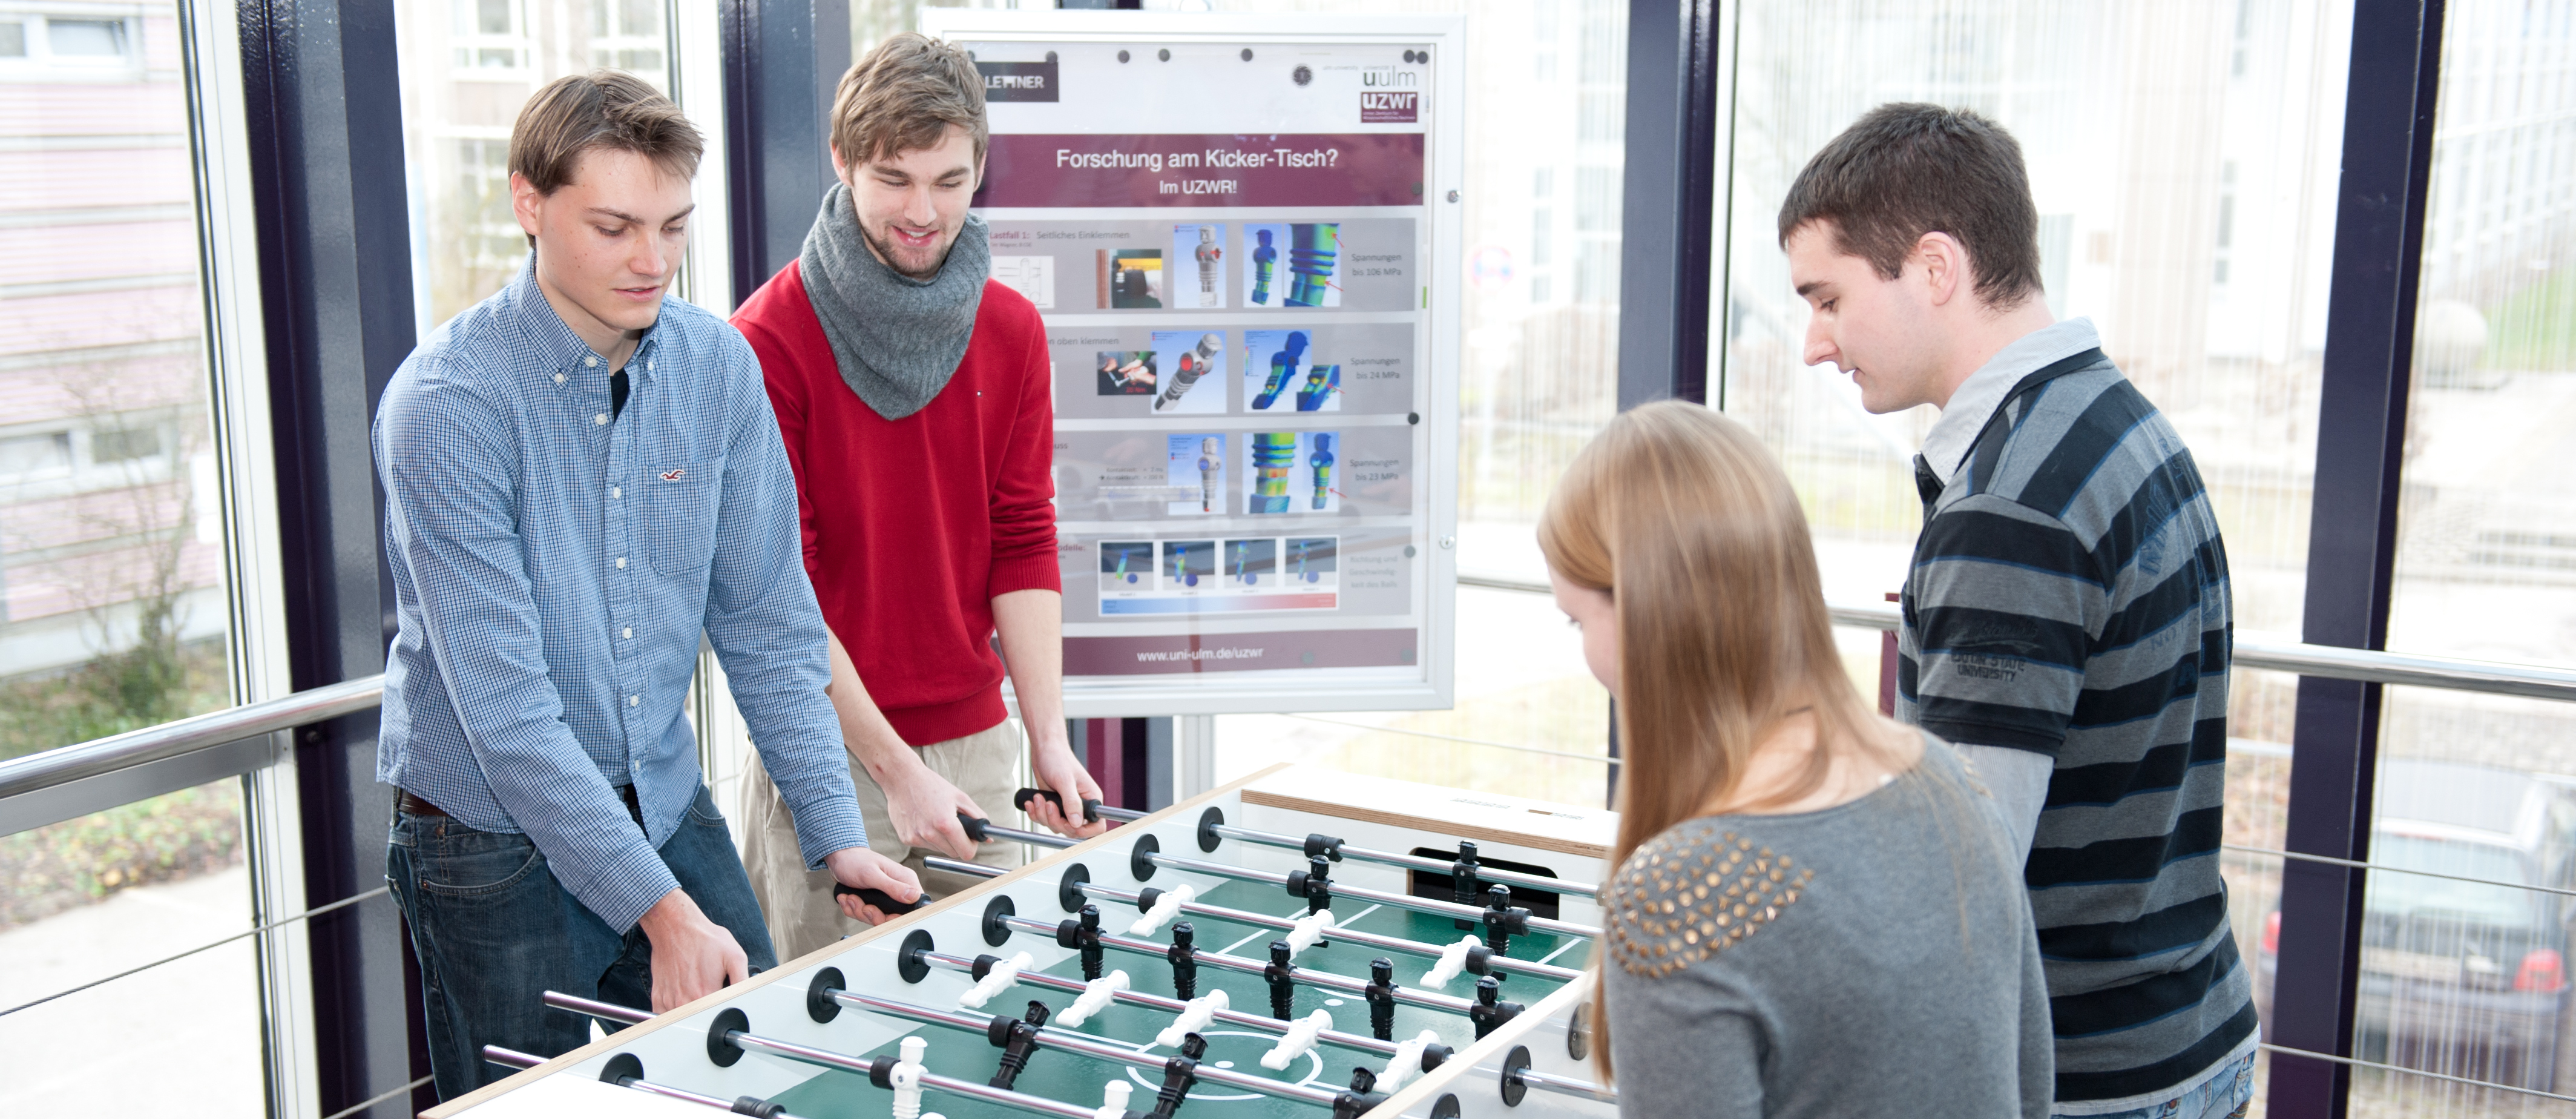
\includegraphics[width=\paperwidth]{tischkicker-wide.jpg}}
        \end{center}

    %\vspace*{1cm}
        \begin{center}
            \textcolor{ecs100}{\hspace{-5cm}\Large  \inserttitle}
        \end{center}
    }


% Das Inhaltsverzeichnis


%%%%%%%%%%%%%%%%%%%%%%%%%%%%%%%%%%%%%%%%%%%%%%%%%%%%%%%%%%%%%%%%%%%%%%%%%%%%%%%%%%%%%%%%%%%
%Ab hier beginnt die Präsentation:
% 1. Folie: Inhaltsverzeichnis
    \begin{frame}
        \frametitle{Inhaltsverzeichnis}
        \tableofcontents
        % [pausesections] % Animation/Einblendung der einzelnen Abschnitte
    \end{frame}

%%%%%%%%%%%%%%%%%%%%%%%%%%%%%%%%%%%%%%%%%%%%%%%%%%%%%%%%%%%%%%%%%%%%%%%%%%%%%%%%%%%%%%%%%%%
%Ab hier beginnt die Präsentation:
    \section{Fachschaft CSE - Wer sind wir?}
    \begin{frame}
        \frametitle{Fachschaft CSE - Wer sind wir?}
        \begin{itemize}
            \setlength{\itemsep}{10pt} %Zeilenabstand ändern
            \item CSE-Studierende aus dem Bachelor und Master, engagieren uns rund um den Studiengang CSE
            \item Wirken wir an der Weiterentwicklung des Studiengangs mit \\(Bsp. \href{https://www.uni-ulm.de/mawi/mawi-cse/gemeinsame-kommission-cse/}{\color{ecs100}Gemeinsame Kommission})
            \item Organisieren verschiedene Events für CSE-Studierende
            \item FS CSE ist nicht eigenständig, sondern ein Teil der FS Mathe \\(s. \href{https://stuve.uni-ulm.de/struktur/satzungen-ordnungen}{\color{ecs100}Organisationssatzung Anhang A})
            \item Treffen uns in der Regel alle zwei Wochen im Vorlesungszeitraum
        \end{itemize}
    \end{frame}
    
    \begin{frame}
        \frametitle{\href{http://cloud.fs-cse.de}{\Mundus~cloud.fs-cse.de}}
        \vfill
        \begin{itemize}
            \item CSE-Cloud mit Material aus älteren Semestern, bspw. Sammlung von Skripten, Übungsaufgaben, Altklausuren(!)
            \vfill
            \item \href{https://stuve.uni-ulm.de/fs-cse/fuer-cseler/cse-cloud}{\color{ecs100}Registrierung} (\textbf{nur} im Uninetz, oder via VPN/webVPN)
            \vfill
            \item Jeder kann in den Ordner \emph{Datenaustausch} Dateien hochladen
            \vfill
            \item In jedem Semester (mind.) einer mit Admin-Rechten, kann direkt an der richtigen Stelle hochladen
        \end{itemize}
        \vfill
    \end{frame}

    \begin{frame}
        \frametitle{ \href{https://stuve.uni-ulm.de/fs-cse/}{\Mundus~stuve.uni-ulm.de/fs-cse/}}
        \begin{center}
            
\includegraphics[width=0.9\textwidth]{bilder/website.jpeg}
        \end{center}
    \end{frame}

    \section{Grundsätzliches}
    \begin{frame}
        \frametitle{Grundsätzliches}
        \vfill
        \begin{center}
            
\includegraphics[width=0.7\paperwidth]{Logos.png}
        \end{center}
        \vfill
        \begin{itemize}
            \item Kooperationsstudiengang der Universität und Technischen Hochschule Ulm
            \vfill
            \item Vorlesungen an verschiedenen Standorten
            \vfill
            \item Verschiedene Vorlesungszeiten (Wahlpflicht)
            \vfill
            \item Zwei Studierendenausweise
            \vfill
            \item Doppeltes Angebot beim Hochschulsport, Orchestern, Auslandsangeboten etc.
            \item Internet - \href{https://www.uni-ulm.de/einrichtungen/kiz/service-katalog/netzwerk-konnektivitaet/wlan/eduroam/}{\color{ecs100}Eduroam} 
        \end{itemize}
        \vfill
    \end{frame}

    \subsection{Standorte}
    \begin{frame}
        \frametitle{Standorte}
        \begin{center}
            \makebox[\textwidth]{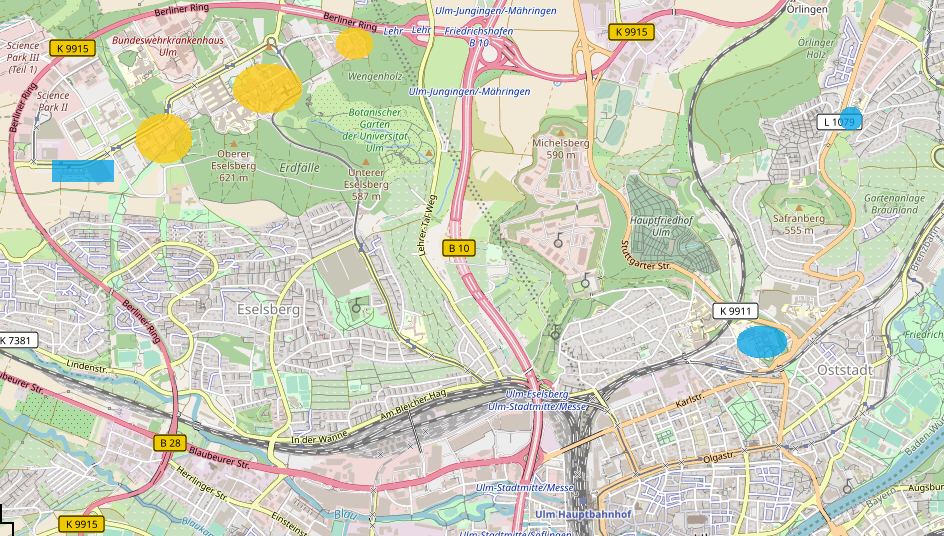
\includegraphics[width=\paperwidth]{Ulm.png}}
        \end{center}
    \end{frame}

    \begin{frame}
        \frametitle{Standorte}
        \begin{center}
            \makebox[\textwidth]{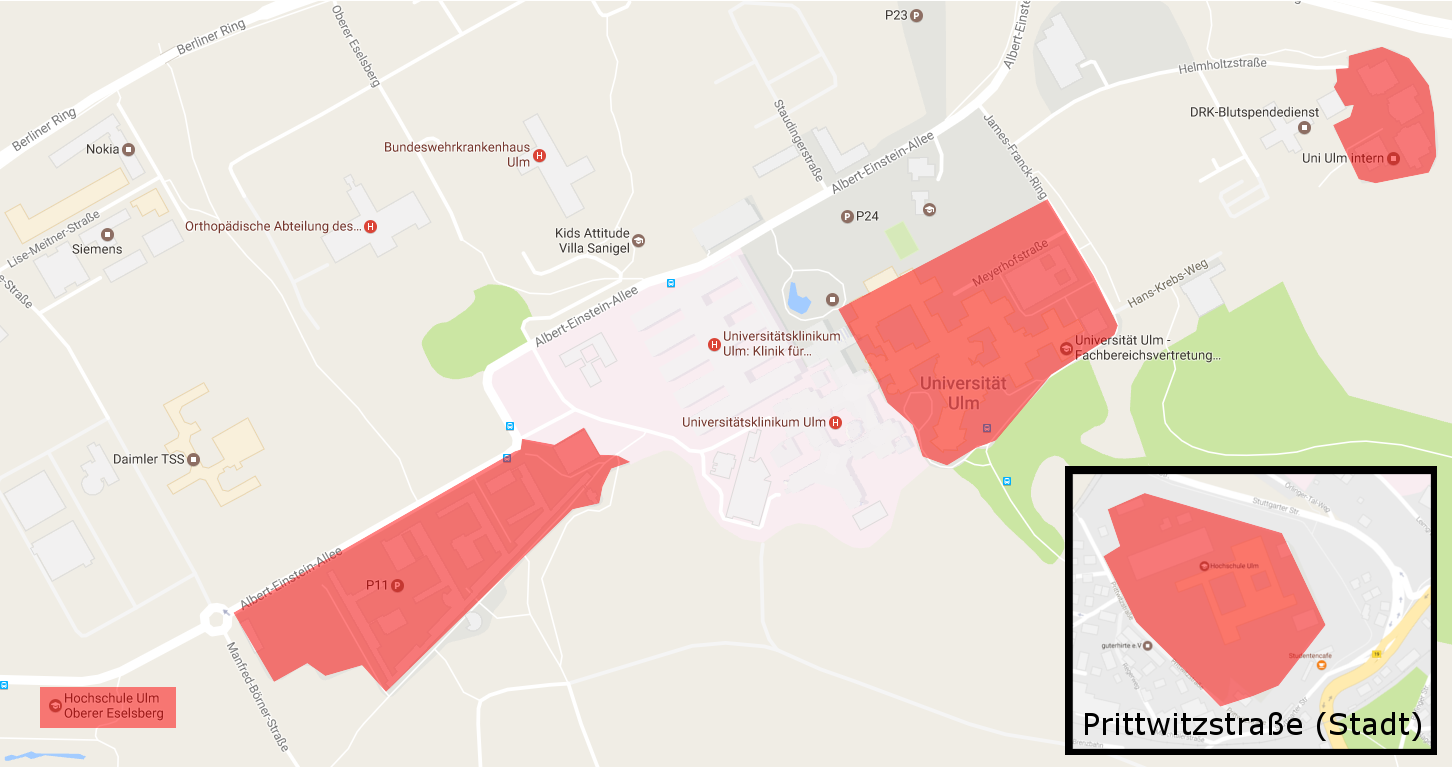
\includegraphics[width=\paperwidth]{karte.png}}
        \end{center}
    \end{frame}


    \subsection{Vorlesungszeiten}
    \begin{frame}
        \frametitle{Vorlesungszeiten}
        \vfill
        \begin{itemize}
            \item Semesterbeginn/-ende
            \vfill
            \begin{itemize}
                \item Uni: 16.10.2023 - 17.02.2024
                \vfill
                \item THU: 04.10.2023 - 26.01.2024
            \end{itemize}
            \vfill
            \item Cum tempore/sine tempore:
            \vfill
            \begin{itemize}
                \item Uni: c.t., die Vorlesung beginnen \emph{Viertel nach}
                \vfill
                \item THU: s.t., die Vorlesungen beginnen \emph{um Punkt}
                \vfill
                \item Bei Prüfungen: Hinweise beachten
            \end{itemize}
        \end{itemize}
        \vfill
    \end{frame}


    \subsection{Studentenausweise}
    \begin{frame}
        \frametitle{Studentenausweise}
        \vfill
        \begin{itemize}
            \item Zwei Studentenausweise mit identischer Matrikelnummer
            \vfill
            \item Verschiedene Konten auf den einzelnen Ausweisen
            \vfill
            \item Verlängerung jedes Semester jeweils an einem Automaten der THU und einem SB-Terminal in der Uni (PIN wird benötigt!)
            \vfill
            \item Kostenlose Fahrt im DING-Netz ab 18h sowie am Wochenende und an Feiertagen
        \end{itemize}
        \vfill
    \end{frame}

    \subsubsection*{Studentenausweis Universität}
    \begin{frame}
        \frametitle{Studentenausweis Universität}
        \vfill
        \begin{itemize}
            \item Zugangskarte zu PC-Pools sowie nachts zur Universität
            \vfill
            \item Bezahlmittel mit drei verschiedenen Konten:
            \vfill
            \begin{itemize}
                \item \textbf{Mensa} - Aufwertung durch Terminals oder am Info-Point), Bezahlen auch in den Mensen der THU möglich
                \vfill
                \item \textbf{Parken} - Aufwertung durch Automaten bei den Parkplätzen
                \vfill
                \item \textbf{Druckkontingent} - Umbuchung am SB-Terminal, 16 Euro pro Kalenderjahr frei
                \vfill
                \item \textbf{Druck- und Kopierkonto} - für Drucker von Ricoh, zusätzlich
            \end{itemize}
            \vfill
            \item Identifikationsmittel bei Prüfungen
        \end{itemize}
        \vfill
    \end{frame}

    \subsubsection*{Studentenausweis Technische Hochschule}
    \begin{frame}
        \frametitle{Studentenausweis Technische Hochschule}
        \vfill
        \begin{itemize}
            \item Bezahlmittel an den Mensen der Technische Hochschule oder Universität
            \vfill
            \item Identifikationsmittel beim Drucken % (10? Euro pro Semester frei)
            \vfill
            \item Zugang zu den \textbf{kostenlosen} Parkplätzen der Technischen Hochschule
            \vfill
            \item Identifikationsmittel bei Prüfungen
        \end{itemize}
        \vfill
    \end{frame}

    \section{Accounts und Portale}
    \begin{frame}
        \frametitle{Accounts und Portale}
        \vfill
        \begin{itemize}
            \item E-Mails
            \vfill
            \begin{itemize}
                \item https://sogo.uni-ulm.de/SOGo/
                \vfill
                \item https://webmail.hs-ulm.de
            \end{itemize}
            \vfill
            \item LSF
            \vfill
            \begin{itemize}
                \item https://campusonline.uni-ulm.de
                \vfill
                \item (https://lsf.verwaltung.hs-ulm.de)
            \end{itemize}
            \vfill
            \item Moodle
            \vfill
            \begin{itemize}
                \item https://moodle.uni-ulm.de
                \vfill
                \item https://moodle-thu.de
            \end{itemize}
        \end{itemize}
        \vfill
    \end{frame}


    \section{Prüfungsanmeldung}
    \begin{frame}
        \frametitle{Prüfungsanmeldung}
        \vfill
        \begin{itemize}
            \item Anmeldung spätestens \textbf{vier Tage vor der Prüfung}
            \vfill
            \item Alle Prüfungen müssen über das Portal der Uni Ulm angemeldet werden, \textbf{nicht} über die Hochschule
            \vfill
            \item Bei Fragen an die \href{https://www.uni-ulm.de/mawi/mawi-cse/studienfachberatung/}{\color{ecs100}\Mundus~Studienfachberatung CSE} wenden
            \vfill
            \begin{itemize}
                \item Beate Mayer (Universität Ulm) - beate.mayer@uni-ulm.de
                \vfill
                \item Kirsten Huss (Hochschule Ulm) - huss@hs-ulm.de
            \end{itemize}
        \end{itemize}
        \vfill
    \end{frame}

    \section{Weitere Tipps \& Tools}
    \begin{frame}
        \frametitle{Weitere Tipps \& Tools}
        \textbf{Tipps:}
        \vfill
        \begin{itemize}
            \item Netzwerk aufbauen – sowohl mit Kommilitonen als auch mit Professoren. Nutzt die (FU)ESE!
            \vfill
            \item Lernen lernen – wie lernst du?
            \vfill
            \item Bafög - bequemes \href{https://www.bafoeg-digital.de/}{\color{ecs100}Online-Portal}, alles digital (nutzt die Online-Ausweisfunktion!). Mehr Infos \href{https://studierendenwerk-ulm.de/bafoeg-finanzen/}{\color{ecs100}hier}.
        \end{itemize}
        \vfill
    \end{frame}

    \begin{frame}
        \frametitle{Weitere Tipps \& Tools}
        \vfill
        \textbf{Tools:}
        \vfill
        \begin{itemize}
            \item \textbf{Anki\,
\includegraphics[height=10pt]{bilder/anki.png}:} Eine nützliche App für Karteikarten.
            \vfill
            \item \textbf{GitHub\,\faIcon{github} (/git):} Eine Cloud-Plattform für deinen Code.
            \vfill
            \item \textbf{Overleaf\,
\includegraphics[height=10pt]{bilder/overleaf.png}:} Eine Online-Plattform für kollaboratives Schreiben und Teilen von LaTeX-Dokumenten.
            \vfill
            \item \textbf{VS Code\,
\includegraphics[height=10pt]{bilder/vs-code.png}:} Ein leistungsstarker Code-Editor mit vielen Erweiterungen für verschiedene Programmiersprachen.
            \vfill
            \item \textbf{Notabilitiy\,
\includegraphics[height=10pt]{bilder/notability.png}:} Eine App zur digitalen Notizen- und Handschriftenerfassung (iPad).
            \vfill
            \item \textbf{Notion\,
\includegraphics[height=10pt]{bilder/notion.png}:} Eine vielseitige Plattform für Notizen und Organisation.
            \vfill
            \item \textbf{Reclaim\,
\includegraphics[height=10pt]{bilder/reclaim.png}:} Eine KI App für automatisierte Terminplanung, die dir bei der effizienten Organisation deines Zeitplans helfen kann.
            \vfill
            \item \textbf{LinkedIn\,\faIcon{linkedin}:} Ein soziales Netzwerk zur beruflichen Vernetzung und Karriereentwicklung. Welche Jobs, Praktika, Auslandsaufenthalte machen oder haben andere (ehemalige) CSE-Studenten gemacht?
        \end{itemize}
        \vfill
    \end{frame}

    \begin{frame}
        \vfill
        \begin{center}
            \huge{Viel Erfolg und Spaß beim Studium!}
            \vfill
            \huge{Noch Fragen?}
        \end{center}
        \vfill
        \begin{flushright}
            
\includegraphics[width=.4\textwidth]{bilder/meme.jpg}
        \end{flushright}
    \end{frame}

\end{document}